\documentclass{article}
\usepackage{fullpage}
%%% Работа с русским языком
\usepackage[T2A]{fontenc}
\usepackage[utf8]{inputenc}
\usepackage[english,russian]{babel}   %% загружает пакет многоязыковой вёрстки
%\usepackage{fontspec}      %% подготавливает загрузку шрифтов Open Type, True Type и др.
%\defaultfontfeatures{Ligatures={TeX},Renderer=Basic}  %% свойства шрифтов по умолчанию
%\setmainfont[Ligatures={TeX,Historic}]{Times New Roman} %% задаёт основной шрифт документа
%\setsansfont{Comic Sans MS}                    %% задаёт шрифт без засечек
%\setmonofont{Courier New}
\usepackage{indentfirst}
\frenchspacing

\usepackage{graphicx}
%\graphicspath{ {images/} }

\usepackage{titlesec} % package to customize chapters, sections and subsections style
%--------------------------------------
\titleformat{\section}{\large\bfseries\centering}{\thesection}{1em}{}
%Hyphenation rules
%--------------------------------------
\usepackage{hyphenat}
\hyphenation{мате-мати-ка восста-навливать}
%--------------------------------------
%%% Дополнительная работа с математикой
\usepackage{amsmath,amsfonts,amssymb,amsthm,mathtools} % AMS
\usepackage{icomma} % "Умная" запятая: $0,2$ --- число, $0, 2$ --- перечисление

%% Перенос знаков в формулах (по Львовскому)
\newcommand*{\hm}[1]{#1\nobreak\discretionary{}
{\hbox{$\mathsurround=0pt #1$}}{}}

\renewcommand{\le}{\ensuremath{\leqslant}}
\renewcommand{\leq}{\ensuremath{\leqslant}}
\renewcommand{\ge}{\ensuremath{\geqslant}}
\renewcommand{\geq}{\ensuremath{\geqslant}}

% Use wide margins, but not quite so wide as fullpage.sty
%\marginparwidth 0.5in
%\oddsidemargin 0.25in
%\evensidemargin 0.25in
%\marginparsep 0.25in
%\topmargin 0.25in
%\textwidth 6in \textheight 8in
% That's about enough definitions

\title{Для Лены}
\author{Ригованов Филипп Юрьевич}
\date{Июль 2015}

\begin{document}

\maketitle
\section*{Вариант № 1.}
\begin{enumerate}

\item % Задача 1
Вычислите сумму последовательности:
$$1-\frac{3}{5}+\frac{9}{25}-\frac{27}{75}+\frac{81}{375}+\ldots$$
Непонятно что здесь за последовательность, видимо тут ошибка в условии, предположим что имелась в виду сумма следующей последовательности:
$$1-\frac{3}{5}+\frac{9}{25}-\frac{27}{125}+\frac{81}{625}+\ldots$$
Решение:

Тогда очевидно последовательность является бесконечно убывающей геометрической последовательностью, со знаменателем $q=-\frac{3}{5}$ и $b_1=1$. Как известно её сумма равна $$S=\frac{b_1}{1-q}=\frac{1}{1+\frac{3}{5}}=\frac{1}{\frac{8}{5}}=\frac{5}{8}=0,625$$
Ответ: $0,625$.

\item % Задача 2
Найдите производную функции:

a) $y=\frac{\cos{x}}{e^x}$

Решение:
$$y'=\left(\frac{\cos{x}}{e^x}\right)'=\left(\cos{x}\cdot e^{-x}\right)'=\cos{x}\cdot\left(e^{-x}\right)'+\left(\cos{x}\right)'\cdot e^{-x}=\cos{x}\cdot\left(-e^{-x}\right)+\left(-\sin{x}\right)\cdot e^{-x}=$$ $$=-e^{-x}\left(\cos{x}+\sin{x}\right)$$

б) $y=x^{11}\cdot\sin{x}$

Решение:
$$y'=\left(x^{11}\cdot\sin{x}\right)'=x^{11}\cdot\left(\sin{x}\right)'+\left(x^{11}\right)'\cdot\sin{x}=x^{11}\cdot\cos{x}+11x^{10}\cdot\sin{x}$$

\item % Задача 3
Найдите промежутки монотонности функции:
$$y=2x^3-3x^2-36x+40$$
Решение:
$$y'=\left(2x^3-3x^2-36x+4\right)'=6x^2-6x-36=6\left(x^2-x-6\right)$$ % =6(x-3)(x+2)

Приравняем производную к нулю и найдём корни уравнения $x^2-x-6=0$:
$$D=(-1)^2-4\cdot1\cdot(-6)=1+24=25$$
$$x_1=\frac{1-\sqrt{25}}{2}=\frac{1-5}{2}=\frac{-4}{2}=-2$$
$$x_2=\frac{1+\sqrt{25}}{2}=\frac{1+5}{2}=\frac{6}{2}=3$$
$y'<0$ при $x\in\left(-2;3\right)$, а значит на этом интервале функция $y$ убывает.

$y'>0$ при $x\in\left(-\infty;-2\right)\cup\left(3;+\infty\right)$, а значит на этих интервалах функция $y$ возрастает.

\item % Задача 4
Найдите точки экстремума:
$$y=x^3-3x^2$$
Решение:
$$y'=\left(x^3-3x^2\right)'=3x^2-3\cdot2x=3x(x-2)$$
$x_1=0$ и $x_2=2$ - корни уравнения $3x(x-2)=0$.

Составим таблицу для нахождения точек экстремума:

\begin{center}
\begin{tabular}{|c|c|c|}
\hline
$x$ & $y'$ & $y$ \\
\hline\hline
$\left(-\infty;0\right)$ & $+$ & $\nearrow$ возрастает \\
\hline
0 & 0 & max\\
\hline
$\left(0;2\right)$ & $-$ & $\searrow$ убывает\\
\hline
2 & 0 & min \\
\hline
$\left(2;+\infty\right)$ & $+$ & $\nearrow$ возрастает \\
\hline
\end{tabular}
\end{center}

Ответ: $x_1=0$ - точка максимума, $x_2=2$ - точка минимума.

\item % Задача 5
Вычислите интеграл:
$$\int{\left(5-e^x+3\cos{x}+x^4\right)dx}$$
Решение:

$$\int{\left(5-e^x+3\cos{x}+x^4\right)dx}=5\int{dx}-\int{e^x dx}+3\int{\cos{x}dx}+\int{x^4dx}=5x-e^x+3\sin{x}+\frac{x^5}{5}+C$$

\item % Задача 6
Найдите корни уравнения:
$$5^{x+1}+3\cdot5^{x-1}-6\cdot5^x+10=0$$
Решение:

Умножим уравнение на 5 и запишем уравнение в следующем виде: $$25\cdot5^x+3\cdot5^x-30\cdot5^x+50=0$$

Пусть $t=5^x$, тогда уравнение, превратившись в линейное, перепишется так: $$25t+3t-30t+50=0$$ откуда $$-2t+50=0$$ $$t=25$$ значит $$5^x=25$$ $$5^x=5^2$$ $$x=2$$

Ответ: 2.

\item % Задача 7
Решите уравнение:
$$\log_2{(2x-18)}+\log_2{(x-9)}=5$$
Решение:
$$\log_2{(2(x-9))}+\log_2{(x-9)}=5$$
$$log_2{2}+\log_2{(x-9)}+\log_2{(x-9)}=5$$
$$2\log_2{(x-9)}=5-1$$
$$\log_2{(x-9)}=2$$
$$\log_2{(x-9)}=\log_2{4}$$
$$x-9=4$$
$$x=13$$
Ответ: 13.

\item % Задача 8
Решите неравенство:
$$\frac{3x-6}{2x^2+5x-3}\le0$$
Решение:

Разложим на множители знаменатель, для этого найдем корни уравнения $2x^2+5x-3=0$ $$D=5^2-4\cdot2\cdot(-3)=25+24=49$$ $$x_1=\frac{-5-\sqrt{49}}{4}=\frac{-12}{4}=-3$$ $$x_2=\frac{-5+\sqrt{49}}{4}=\frac{2}{4}=0,5$$
Значит исходное неравенство, предварительно разделив обе части на 3, можно переписать в виде:
$$\frac{x-2}{(x+3)(x-0,5)}\le0$$

В таком виде для решения неравенства уже удобно применить метод интервалов:

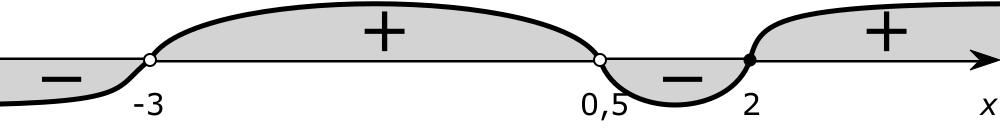
\includegraphics[width=\textwidth]{1_8.png}

Ответ: $x\in\left(-\infty;-3\right)\cup\left(0,5;2\right]$.

\item % Задача 9
В вазе лежат яблоки: 12 жёлтых и 6 красных. Сколькими способами можно взять из вазы 4 жёлтых и 2 красных яблока?

Решение:

Число способов выбрать 4 жёлтых яблока из 12 равно $$C_{12}^4=\frac{12!}{4!\cdot8!}=\frac{9\cdot10\cdot11\cdot12}{2\cdot3\cdot4}=9\cdot5\cdot11=495$$
Число способов выбрать 2 красных яблока из 6 равно
$$C_{6}^2=\frac{6!}{2!\cdot4!}=\frac{5\cdot6}{2}=15$$
Для каждого из вариантов выбора жёлтых яблок можно взять любой из вариантов выбора красных, значит нужно применить правило произведения и искомое число способов равно $495\cdot15=7425$.

Ответ: 7425.

\item % Задача 10
В сборнике билетов по биологии всего 25 билетов, в двух из них встречается вопрос о грибах. На экзамене школьнику достаётся один случайно выбранный билет из этого сборника. Найдите вероятность того, что в этом билете не будет вопроса о грибах.

Решение:

По формуле классической вероятности $P(A)=\frac{m}{n}$, где общее число элементарных исходов $n=25$, а число благоприятных исходов $m=25-2=23$ значит $$P(A)=\frac{23}{25}=0,92$$

Ответ: $0,92$.

\end{enumerate}
\section*{Вариант № 2.}
\begin{enumerate}

\item % Задача 1
Вычислите сумму последовательности:
$$1-\frac{2}{3}+\frac{4}{9}-\frac{8}{27}+\frac{16}{81}-\ldots$$
Решение:

Очевидно последовательность является бесконечно убывающей геометрической последовательностью, со знаменателем $q=-\frac{2}{3}$ и $b_1=1$. Как известно её сумма равна $$S=\frac{b_1}{1-q}=\frac{1}{1+\frac{2}{3}}=\frac{1}{\frac{5}{3}}=\frac{3}{5}=0,6$$
Ответ: $0,6$.
\item % Задача 2
Найдите производную функции:

a) $y=\frac{3^x}{\sin{x}}$

Решение:

$$y'=\left(\frac{3^x}{\sin{x}}\right)'=\frac{(3^x)'\sin{x}-3^x(\sin{x})'}{\sin^2{x}}=\frac{3^x\cdot\ln{3}\cdot\sin{x}-3^x\cdot\cos{x}}{\sin^2{x}}=\frac{3^x}{\sin{x}}\cdot(\ln{3}-\ctg{x})$$

б) $y=x^{7}\cdot\cos{x}$

Решение:

$$y'=\left(x^7\cdot\cos{x}\right)'=(x^7)'\cdot\cos{x}+x^7\cdot(\cos{x})'=7x^6\cos{x}-x^7\sin{x}$$

\item % Задача 3
Найдите промежутки монотонности функции:
$$y=x^3-2x^2+x-2$$
Решение:
$$y'=\left(x^3-2x^2+x-2\right)'=3x^2-4x+1$$
Приравняем производную к нулю и найдём корни уравнения $3x^2-4x+1=0$:
$$D=(4)^2-4\cdot3\cdot1=16-12=4$$
$$x_1=\frac{4-\sqrt{4}}{2\cdot3}=\frac{4-2}{2\cdot3}=\frac{2}{2\cdot3}=\frac{1}{3}$$
$$x_2=\frac{4+\sqrt{4}}{2\cdot3}=\frac{4+2}{6}=\frac{6}{6}=1$$
$y'<0$ при $x\in\left(\frac{1}{3};1\right)$, а значит на этом интервале функция $y$ убывает.

$y'>0$ при $x\in\left(-\infty;\frac{1}{3}\right)\cup\left(1;+\infty\right)$, а значит на этих интервалах функция $y$ возрастает.
\item % Задача 4
Найдите точки экстремума:
$$y=x^3+3x^2-6$$
Решение:
$$y'=\left(x^3+3x^2-6\right)'=3x^2+3\cdot2x=3x(x+2)$$
$x_1=-2$ и $x_2=0$ - корни уравнения $3x(x+2)=0$.

Составим таблицу для нахождения точек экстремума:

\begin{center}
\begin{tabular}{|c|c|c|}
\hline
$x$ & $y'$ & $y$ \\
\hline\hline
$\left(-\infty;-2\right)$ & $+$ & $\nearrow$ возрастает \\
\hline
-2 & 0 & max\\
\hline
$\left(-2;0\right)$ & $-$ & $\searrow$ убывает\\
\hline
0 & 0 & min \\
\hline
$\left(0;+\infty\right)$ & $+$ & $\nearrow$ возрастает \\
\hline
\end{tabular}
\end{center}

Ответ: $x_1=-2$ - точка максимума, $x_2=0$ - точка минимума.
\item % Задача 5
Вычислите интеграл:
$$\int{\left(1+3e^x-4\cos{x}+x^3\right)dx}$$
Решение:

$$\int{\left(1+3e^x-4\cos{x}+x^3\right)dx}=\int{dx}+3\int{e^x dx}-4\int{\cos{x}dx}+\int{x^3dx}=x+3e^x-4\sin{x}+\frac{x^4}{4}+C$$

\item % Задача 6
Найдите корни уравнения:
$$2\cdot3^{x+1}-6\cdot3^{x-1}-3^x=9$$
Решение:

Перепишем уравнение в следующем виде: $$6\cdot3^{x}-2\cdot3^{x}-3^x=9$$

Пусть $t=3^x$, тогда уравнение, превратившись в линейное, перепишется так: $$6t-2t-t=9$$ откуда $$3t=9$$ $$t=3$$ значит $$3^x=3$$ $$3^x=3^1$$ $$x=1$$

Ответ: 1.

\item % Задача 7
Решите уравнение:
$$\log_3{(x-7)}+\log_3{(x+1)}=2$$
Решение:

Выпишем ОДЗ уравнения: из определения логарифмической функци одновременно должно быть $x-7>0$ и $x+1>0$ или  одновременно $x>7$ и $x>-1$, а это значит просто $x>7$.
$$\log_3{(x-7)}+\log_3{(x+1)}=2$$
$$\log_3{(x-7)(x+1)}=2$$
$$\log_3{(x-7)(x+1)}=\log_3{9}$$
$$(x-7)(x+1)=9$$
$$x^2-6x-7=9$$
$$x^2-6x-16=0$$
$$D=(-6)^2-4\cdot1\cdot(-16)=36+64=100$$
$$x_1=\frac{6-\sqrt{100}}{2}=\frac{6-10}{2}=\frac{-4}{2}=-2$$
$$x_2=\frac{6+\sqrt{100}}{2}=\frac{6+10}{2}=\frac{16}{2}=8$$
Но $x_1=-2$ не попадает в ОДЗ $x>7$, значит уравнение имеет единственный корень $x=8$.

Ответ: 8.
\item % Задача 8
Решите неравенство:
$$\frac{3x-5}{x^2+5x-14}\ge0$$
Решение:

Разложим на множители знаменатель, для этого найдем корни уравнения $x^2+5x-14=0$ $$D=5^2-4\cdot1\cdot(-14)=25+56=81$$ $$x_1=\frac{-5-\sqrt{81}}{2}=\frac{-14}{2}=-7$$ $$x_2=\frac{-5+\sqrt{81}}{2}=\frac{4}{2}=2$$
Значит исходное неравенство, предварительно разделив обе части на 3, можно переписать в виде:
$$\frac{x-\frac{5}{3}}{(x+7)(x-2)}\ge0$$

В таком виде для решения неравенства уже удобно применить метод интервалов:

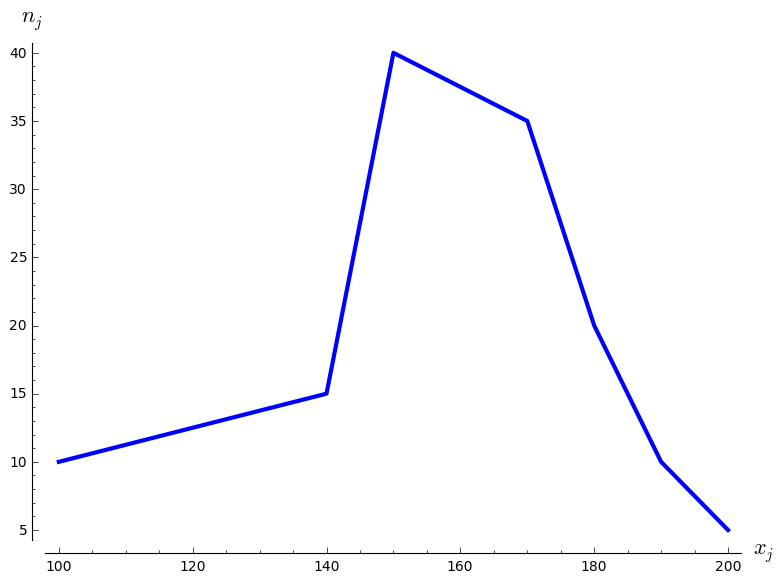
\includegraphics[width=\textwidth]{2_8.png}

Ответ: $x\in\left(-7;\frac{5}{3}\right]\cup\left(2;+\infty\right)$.

\item % Задача 9
В вазе лежат яблоки: 10 зелёных и 5 красных. Сколькими способами можно взять из вазы 2 зелёных и 3 красных яблока?

Решение:

Число способов выбрать 2 зелёных яблока из 10 равно $$C_{10}^2=\frac{10!}{2!\cdot8!}=\frac{9\cdot10}{2}=9\cdot5=45$$
Число способов выбрать 3 красных яблока из 5 равно
$$C_{5}^3=\frac{5!}{3!\cdot2!}=\frac{4\cdot5}{2}=10$$
Для каждого из вариантов выбора зелёных яблок можно взять любой из вариантов выбора красных, значит нужно применить правило произведения и искомое число способов равно $45\cdot10=450$.

Ответ: 450.

\item % Задача 10
В сборнике билетов по биологии всего 25 билетов, в двух из них встречается вопрос о грибах. На экзамене школьнику достаётся один случайно выбранный билет из этого сборника. Найдите вероятность того, что в этом билете будет вопрос о грибах.

Решение:

По формуле классической вероятности $P(A)=\frac{m}{n}$, где общее число элементарных исходов $n=25$, а число благоприятных исходов $m=2$ значит $$P(A)=\frac{2}{25}=0,08$$

Ответ: $0,08$.

\end{enumerate}
\end{document}
